The next model we consider is an agent-based model. Each individual in the population can be in either of 7 states discussed above: susceptible, exposed, infected, hospitalized, funeral, recovered or dead. The flow between two states is a  probability of transition from one state to another for a typical individual. We represent our model in Figure~\ref{ABM}. In each time step a typical individual who is susceptible to contracting a virus can either transition to exposed state with probability $p_{SE}$ or stay susceptible with probability $p_{SS}$. An individual in the exposed state transitions to infected with probability $p_{EI}$ and stays exposed with probability $p_{EE}$. An individual who is infected can stay infected, recover, go to a hospital or die and transition to funeral state with probabilities $p_{II},\, p_{IR},\, p_{IH}$ and $p_{IF}$ respectively. Recovery is considered a terminal state so individuals in this state stay in it for the remaining duration of the simulation. Hospitalized individuals may stay hospitalized, transition to recovered or funeral with probabilities $p_{HH}, \, p_{HR}$ and $p_{HF}$. We assume that the individual who dies from Ebola remains infectious through the duration of the entire burial ceremony and no precautions are taken against disease transmission. Safely buried individuals are considered dead and noninfectious and remain in this state for the remaining time of the simulation.  

%  \begin{tikzpicture}[node distance=2cm, font=\tiny]
%        \node [draw, terminal]  (start) at (0,0) {Start};
%        \node [draw, predproc, right of= start] (acquire)(write) {Acquire Image};
%
%%% paths
%    \draw[->](work) -- node[above]{yes}(end);
%    \end{tikzpicture}
\begin{figure}[h!]
\begin{center}
\begin{tikzpicture}[->,>=stealth',shorten >=1pt,auto,node distance=3cm,
  thick,main node/.style={circle,fill=blue!20,draw,font=\sffamily\Large\bfseries}]

  \node[main node] (1) {S};
  \node[main node] (2) [right of=1] {E};
  \node[main node] (3) [right of=2] {I};
  \node[main node] (4) [right of=3] {R};
    \node[main node] (5) [below left of=3] {D};
      \node[main node] (6) [below right of=3] {F};
        \node[main node] (7) [right of=6] {H};

  \path[every node/.style={font=\sffamily\small}]
    (1)
        edge node {$p_{SE}$} (2)
        edge [loop above] node {$p_{SS}$} (1)
    (2) 
        edge node {$p_{EI}$} (3)
         edge [loop above] node {$p_{EE}$} (2)
      
    (3) 
       edge node {$p_{IR}$} (4)
       edge node[left] {$p_{IF}$} (6)
       edge node {$p_{IH}$} (7)
        edge [loop above] node {$p_{II}$} (3)
    (4)
         edge [loop above] node {$p_{RR}$} (4)
       
(6) edge node{$p_{FD}$} (5) 
edge [loop below] node {$p_{FF}$} (6)     
(7) edge node[right]{$p_{HR}$} (4) 
edge [loop below] node {$p_{HH}$} (7)
  (7) edge node{$p_{HF}$} (6)      
 (5) edge [loop below] node {$p_{DD}$} (5)
        ;
        
\end{tikzpicture}
\end{center}
\caption{Spread of the disease: Agent-based model. Each node represents a typical individual's state. An individual can transition to a state to which he is connected by a directed arc with a probability specified on an arc.}
\label{ABM}
\end{figure}
Let

\begin{itemize}
\item[]$t_{IP}$ be the incubation period, i.e. time during which the individual has the virus in his body but does not yet show severe symptoms
\item[] $t_{ID}$ infection duration time after the onset of severe symptoms
\item[] $t_{H}$ time to hospitalization after manifestation of severe symptoms
\item[] $t_{IF}$ time from the onset of severe symptoms to funeral
\item[] $t_{HF}$ time from patient's arrival at the hospital to funeral
\item[] $t_{HR}$ time from patient's arrival at the hospital to recovery
\item[] $t_{DF}$ duration of traditional funeral
\item[] $N$  total number of individuals in a population
\item[] $N_{I}$  total number of individuals in the infected state
\item[] $N_{H}$  total number of individuals in the hospitalized state
\item[] $N_{F}$  total number of individuals in the funeral state
\item[] $\beta_{I}$ rate at which the disease spreads during an interaction with an infected person
\item[] $\beta_{H}$ rate at which the disease spreads during an interaction with a hospitalized person
\item[] $\beta_{F}$ rate at which the disease spreads during an interaction with a person who is in the funeral state
\end{itemize}
We define the individual's probability of transition for each state as

\begin{subequations}
\begin{alignat}{1}

\end{alignat}
\end{subequations}
\subsection{Simulation}
We consider a population of size 1000 with 999 individuals starting in a susceptible state and 1 individual in the exposed state. Numeric probabilities of an individual transitioning from each state are recorded in Table~\ref{tab:probabilities}. We repeat the process 100 times and record the average outcome.  
Since this model is not deterministic, each time we see a different outcome. We define an outbreak as an event in which 1\% of the population or more contracts the disease. If only one individual is exposed to the disease in a population of 1000, there is about 30\% chance that the outbreak will not happen (27/100 cases). However, once the cumulative proportion of the exposed individuals reaches 1\%, the virus will affect more than 90\% of the population. A histogram for simulation outcomes is depicted in Figure~\ref{fig:Hist}.
%
%
% HERE IS THE PROBABILITY TRANSITION TABLE
%
%
%
%
\begin{table}[h!]
\caption{Agent-Model Parameters for Ebola Epidemic in Liberia Before and After the International Intervention} % title of Table
\centering % used for centering table
\begin{tabular}{c c c c} 
\hline\hline %inserts double horizontal lines
Parameter & Definition&  Liberia Before Intervention  & Liberia After Intervention \\ %[0.5ex] 
& & (Mar 2014 to Sept 2014) &  (Sept 2014 to Jul 2015) \\ %[0.5ex] % inserts table
% inserts table
%heading
\hline % inserts single horizontal line
$p_{SE}$	 &$\beta_I N_{I}/N+\beta_H N_{H}/N+\beta_F  N_F/ N$ 	& \textbf{DYNAMIC}	 & \textbf{DYNAMIC} \\ 
$p_{SS}$ 	& $1-p_{SE}$													 & \textbf{COMPUTE}8	 & \textbf{COMPUTE}  \\ 
$p_{EE}$ 	& $1-1/t_{IP}$ 												& 0.9091 			& 0.9091  \\ 
$p_{EI}$ 	& $1/t_{IP}$ 												&0.0909			 & 0.0909  \\ 
$p_{II}$ 	& $1/t_{ID}$ 												& 0.1 				& 0.1  \\ 
$p_{IH}$	 & $1/t_{H}$ 												&0.2227 			& 0.2160  \\ 
$p_{IF}$ 	& $1/t_{IF}$ 												& 0.125 			& 0.125  \\ 
$p_{IR}$ 	& $1-p_{II}-p_{IH}-p_{IF}$ 											&0.5523 			& 0.559  \\ 
$p_{HF}$ 	& $1/t_{HF}$												& 0.2849 			& 0.2849 \\ 
$p_{HR}$ 	& $1/t_{HR}$ 												&0.1815 			& 0.1815 \\ 
$p_{HH}$ 	& $1-p_{HF}-p_{HR}$ 												& 0.5336			& 0.5336  \\ 
$p_{FF}$ 	& $1/t_{DF}$ 												&  0.5 			& 0.5 \\ 
$p_{FD}$ 	& $1-p_{FF}$													 & 0.5 			& 0.5  \\ 
$p_{RR}$ 	& 1															& 1 				& 1  \\ 
$p_{DD}$ 	& 1															&1				 & 1 \\ [1ex] 
\hline 
\end{tabular}
\label{tab:probabilities}
\end{table}

\begin{figure}
\begin{center}
\includegraphics[scale=0.5]{N1000Hist.eps}
\end{center}
\caption{Histogram showing the outcome of 100 simulations.}
\label{fig:Hist}
\end{figure}


%%%%%%%%%%%%%%%%%%%%%%%%%%%%%%%%%%%%
% figure N1000Hist.eps
%%%%%%%%%%%%%%%%%%%%%%%%%%%%%%%%%%%%
We note that the simulations reach their stationary state before $t = 500$. We plot the result of 100 simulations. In many cases we don't observe an outbreak of Ebola. However there are many cases which show catastrophic disease. In the disastrous case, on average, 95\% of people get the disease and 76\% of people die from it, as presented in Figure~\ref{fig:Scatter}. 

%%%%%%%%%%%%%%%%%%%%%%%%%%%%%%%%%%%%
% figure N1000Scatter.eps
%%%%%%%%%%%%%%%%%%%%%%%%%%%%%%%%%%%%
 
\begin{figure}
\begin{center}
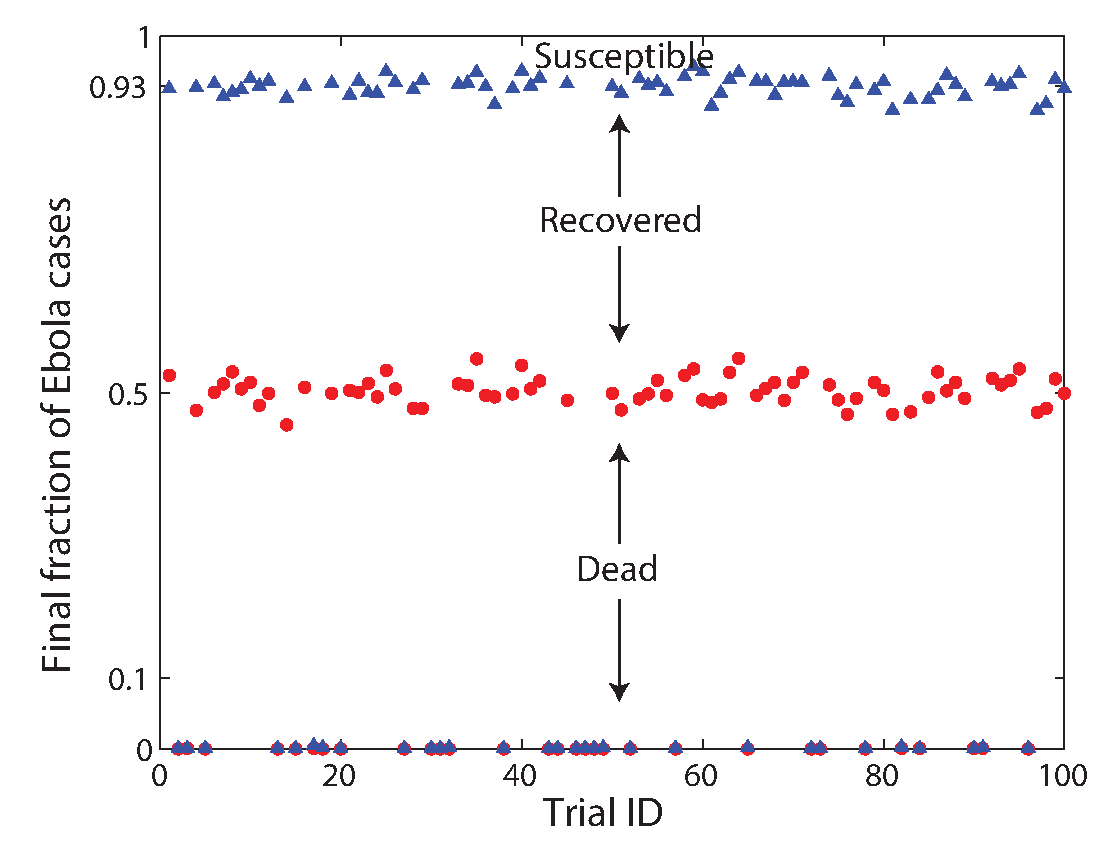
\includegraphics[scale=0.5]{N1000Scatter.eps}
\end{center}
\caption{Scatter plot showing the proportion of population that contracts the disease and the proportion of the population that dies due to the disease for a population size 1000}
\label{fig:Scatter}
\end{figure}

%%%%%%%%%%%%%%%%%%%%%%%%%%%%%%%%%%%%
% figure N1000Scatter.eps
%%%%%%%%%%%%%%%%%%%%%%%%%%%%%%%%%%%%

If there is no outbreak, the infected agent may or may not infect another agent in the population. However, most people remain in the  susceptible state because the infected individual recovers or dies before he infects enough people to cause an outbreak. The number of people who get Ebola is low, so all seven states stay relatively constant over time. %Illustration of this case is presented in Figure~\ref{fig:NoOutbreak}.
%\begin{figure}
%\begin{center}
%\includegraphics[scale=0.8]{NoOutbreak.eps}
%\end{center}
%\caption{No outbreak realization of the outbreak process}
%\label{fig:NoOutbreak}
%\end{figure}

%%%%%%%%%%%%%%%%%%%%%%%%%%%%%%%%%%%%
% figure NoOutbreak.eps
%%%%%%%%%%%%%%%%%%%%%%%%%%%%%%%%%%%%

On the other hand, if the infected agent contacts many people during the time he is infected (I), hospitalized (H), or in a funeral state (F) before he dies or recovers, there is a an outbreak of the disease. A typical outbreak is depicted in Figure~\ref{fig:Outbreak}. The proportion of agents who contract the disease grows exponentially until $t = 125$. That is also the time at which the proportion of population  in states I, H, and F is the highest. After that, the population does not have enough susceptible agents to spread the disease causing the proportion of exposed agents to decrease. The proportion of agents in I, H, and F decreases as well. Around $t = 180$ the proportion of the population is states I, H, and F is zero; the proportion of the population in state S does not decrease, i.e. no agents get Ebola. At this point, all agents remain in S, R or D and an equilibrium is reached (stable fixed point). As we showed before, on average, 5\% of agents stay in state S, 19\% of agents stay in R, and 76\% of agents stay in D. 
%%%%%%%%%%%%%%%%%%%%%%%%%%%%%%%%%%%%
% figure Outbreak.eps
%%%%%%%%%%%%%%%%%%%%%%%%%%%%%%%%%%%%
\begin{figure}
\begin{center}
\includegraphics[scale=0.8]{Outbreak.eps}
\end{center}
\caption{Realization in which outbreak occurs}
\label{fig:Outbreak}
\end{figure}

%%%%%%%%%%%%%%%%%%%%%%%%%%%%%%%%%%%%
% figure Outbreak.eps
%%%%%%%%%%%%%%%%%%%%%%%%%%%%%%%%%%%%


\textbf{Choose how you want to word it; Maybe move description to caption of the figure. Also need to cite only once. Either at the beginning or later}.
We plot a phase portrait for the proportion of agents who never got infected and are in S vs. the proportion of agents who contracted the disease (both D and R) as time progresses.The result is presented in Figure~\ref{fig:PhasePortraitABM}. On the horizontal axis, we put the ratio of S to the total population and on the vertical axis - the ratio of D plus R to the total population.  When $t = 0$, one agent is in state E and 99.9\% of agents are in S. All other states contain no agents. About 30\% of th time, there is no severe outbreak. In such case, only few people get Ebola. As time goes by there are only few transitions between states and a stationary point is reached within a few time steps. However, if there is an outbreak, the trajectory gradually moves to its equilibrium state. On average, the equilibrium occurs at $(S, R+ D) = (0.05, 0.95)$. We conduct ten experiments and plot their trajectories on the same graph, presented in Figure~\ref{fig:PhasePortraitABM}. Because the total proportion of people in the population is one, the equilibria in different experiments lie on the $x + y = 1$ line. The system starts at $(S, [R]+[D]) = (0.999, 0)$, a point that is close to this line. In case of an outbreak, the distance between the point on a trajectory at any time $t$ and the point on an $x+y=1$ line represents \textb{the proportion?} of agents in the transient states: E, I, H and F. 

%%%%%%%%%%%%%%%%%%%%%%%%%%%%%%%%%%%%
% figure PhasePortrait.eps
%%%%%%%%%%%%%%%%%%%%%%%%%%%%%%%%%%%%
\begin{figure}[h!]
\begin{center}
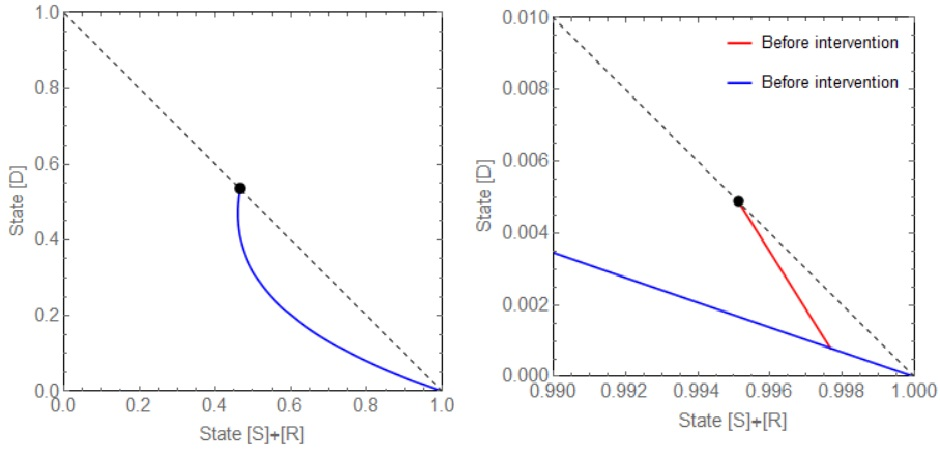
\includegraphics[scale=0.5]{PhasePortrait.eps}
\end{center}
\caption{Phase portrait: proportion of the population who are in susceptible state vs. population of the population who contracted Ebola for different uncertainty realizations.}
\label{fig:PhasePortraitABM}
\end{figure}

%%%%%%%%%%%%%%%%%%%%%%%%%%%%%%%%%%%%
% figure PhasePortrait.eps
%%%%%%%%%%%%%%%%%%%%%%%%%%%%%%%%%%%%

As in the system dynamic approach, we perform an intervention in the agent-based model. Because the scale in the two models is different, we start the intervention if we see an outbreak, i.e. when 1\% of agents are in state E. At the beginning of intervention, we change the three $\beta$s, contact rates. Our results, presented in Figure~\ref{fig:Intervention}, show that if we start the intervention at 1\% of population having Ebola, 4\% of agents get the disease, 1\% of agents recover and 3\% of agents die. This is a significant improvement over the disastrous results of an outbreak without intervention. 

%%%%%%%%%%%%%%%%%%%%%%%%%%%%%%%%%%%%
% figure InterventionZoomIn.eps
%%%%%%%%%%%%%%%%%%%%%%%%%%%%%%%%%%%%

\begin{figure}[h!]
\begin{center}
\includegraphics[scale=0.8]{InterventionZoomIn.eps}
\end{center}
\caption{Effect of Intervention on the spread of the disease }
\label{fig:Intervention}
\end{figure}

%%%%%%%%%%%%%%%%%%%%%%%%%%%%%%%%%%%%
% figure InterventionZoomIn.eps
%%%%%%%%%%%%%%%%%%%%%%%%%%%%%%%%%%%%

We examine the effect of the population size on the outcome of the agent-based model. Aside from $N = 1000$, we set the total population to be $N = 100$ and $5000$. The results are presented in Figure~\ref{fig:VarPopSize}. When we increase the population size, although the average of final S, D, and R states stay the same, the standard deviations of these quantities are smaller in larger systems. The bands of agents who get Ebola and die becomes narrower as population size increases. This suggests that the system becomes more stable. An important implication of this result is that the predicted outcome is more reliable for larger systems.





%%%%%%%%%%%%%%%%%%%%%%%%%%%%%%%%%%%%
%%%%%%%%%%%%%%%%%%%%%%%%%%%%%%%%%%%%
%%%%%%%%%%%%%%%%%%%%%%%%%%%%%%%%%%%%









